\documentclass[11pt,fleqn, oneside,openany]{book} % Default font size and left-justified equations

% use this list: https://www.educative.io/blog/google-coding-interview

%%%%%%%%%%%%%%%%%%%%%%%%%%%%%%%%%%%%%%%%%%%%
%               Structure
%%%%%%%%%%%%%%%%%%%%%%%%%%%%%%%%%%%%%%%%%%%%
%%%%%%%%%%%%%%%%%%%%%%%%%%%%%%%%%%%%%%%%%
% The Legrand Orange Book
% Structural Definitions File
% Version 2.0 (9/2/15)
%
% Original author:
% Mathias Legrand (legrand.mathias@gmail.com) with modifications by:
% Vel (vel@latextemplates.com)
% 
% This file has been downloaded from:
% http://www.LaTeXTemplates.com
%
% License:
% CC BY-NC-SA 3.0 (http://creativecommons.org/licenses/by-nc-sa/3.0/)
%
%%%%%%%%%%%%%%%%%%%%%%%%%%%%%%%%%%%%%%%%%

%----------------------------------------------------------------------------------------
%	VARIOUS REQUIRED PACKAGES AND CONFIGURATIONS
%----------------------------------------------------------------------------------------

\usepackage[top=3cm,bottom=3cm,left=3cm,right=3cm,headsep=10pt,a4paper]{geometry} % Page margins

\usepackage{graphicx} % Required for including pictures
\graphicspath{{images/}} % Specifies the directory where pictures are stored

\usepackage{lipsum} % Inserts dummy text

\usepackage{tikz} % Required for drawing custom shapes

\usepackage[english]{babel} % English language/hyphenation

\usepackage{enumitem} % Customize lists
\setlist{nolistsep} % Reduce spacing between bullet points and numbered lists

\usepackage{booktabs} % Required for nicer horizontal rules in tables

\usepackage{xcolor} % Required for specifying colors by name
\definecolor{ocre}{RGB}{243,102,25} % Define the orange color used for highlighting throughout the book

%----------------------------------------------------------------------------------------
%	FONTS
%----------------------------------------------------------------------------------------

\usepackage{avant} % Use the Avantgarde font for headings
%\usepackage{times} % Use the Times font for headings
\usepackage{mathptmx} % Use the Adobe Times Roman as the default text font together with math symbols from the Sym­bol, Chancery and Com­puter Modern fonts

\usepackage{microtype} % Slightly tweak font spacing for aesthetics
\usepackage[utf8]{inputenc} % Required for including letters with accents
\usepackage[T1]{fontenc} % Use 8-bit encoding that has 256 glyphs

%----------------------------------------------------------------------------------------
%	BIBLIOGRAPHY AND INDEX
%----------------------------------------------------------------------------------------

\usepackage[citestyle=numeric,sorting=nyt,sortcites=true,autopunct=true,babel=hyphen,hyperref=true,abbreviate=false,backref=true,backend=biber]{biblatex}
\addbibresource{sources/bibliography.bib}
\defbibheading{bibempty}{}

\usepackage{calc} % For simpler calculation - used for spacing the index letter headings correctly
\usepackage{makeidx} % Required to make an index
\makeindex % Tells LaTeX to create the files required for indexing

%----------------------------------------------------------------------------------------
%	MAIN TABLE OF CONTENTS
%----------------------------------------------------------------------------------------

\usepackage{titletoc} % Required for manipulating the table of contents

\contentsmargin{0cm} % Removes the default margin

% Part text styling
\titlecontents{part}[0cm]
{\addvspace{20pt}\centering\large\bfseries}
{}
{}
{}

% Chapter text styling
\titlecontents{chapter}[1.25cm] % Indentation
{\addvspace{12pt}\large\sffamily\bfseries} % Spacing and font options for chapters
{\color{ocre!60}\contentslabel[\Large\thecontentslabel]{1.25cm}\color{ocre}} % Chapter number
{\color{ocre}}  
{\color{ocre!60}\normalsize\;\titlerule*[.5pc]{.}\;\thecontentspage} % Page number

% Section text styling
\titlecontents{section}[1.25cm] % Indentation
{\addvspace{3pt}\sffamily\bfseries} % Spacing and font options for sections
{\contentslabel[\thecontentslabel]{1.25cm}} % Section number
{}
{\hfill\color{black}\thecontentspage} % Page number
[]

% Subsection text styling
\titlecontents{subsection}[1.25cm] % Indentation
{\addvspace{1pt}\sffamily\small} % Spacing and font options for subsections
{\contentslabel[\thecontentslabel]{1.25cm}} % Subsection number
{}
{\ \titlerule*[.5pc]{.}\;\thecontentspage} % Page number
[]

% List of figures
\titlecontents{figure}[0em]
{\addvspace{-5pt}\sffamily}
{\thecontentslabel\hspace*{1em}}
{}
{\ \titlerule*[.5pc]{.}\;\thecontentspage}
[]

% List of tables
\titlecontents{table}[0em]
{\addvspace{-5pt}\sffamily}
{\thecontentslabel\hspace*{1em}}
{}
{\ \titlerule*[.5pc]{.}\;\thecontentspage}
[]

%----------------------------------------------------------------------------------------
%	MINI TABLE OF CONTENTS IN PART HEADS
%----------------------------------------------------------------------------------------

% Chapter text styling
\titlecontents{lchapter}[0em] % Indenting
{\addvspace{15pt}\large\sffamily\bfseries} % Spacing and font options for chapters
{\color{ocre}\contentslabel[\Large\thecontentslabel]{1.25cm}\color{ocre}} % Chapter number
{}  
{\color{ocre}\normalsize\sffamily\bfseries\;\titlerule*[.5pc]{.}\;\thecontentspage} % Page number

% Section text styling
\titlecontents{lsection}[0em] % Indenting
{\sffamily\small} % Spacing and font options for sections
{\contentslabel[\thecontentslabel]{1.25cm}} % Section number
{}
{}

% Subsection text styling
\titlecontents{lsubsection}[.5em] % Indentation
{\normalfont\footnotesize\sffamily} % Font settings
{}
{}
{}

%----------------------------------------------------------------------------------------
%	PAGE HEADERS
%----------------------------------------------------------------------------------------

\usepackage{fancyhdr} % Required for header and footer configuration

\pagestyle{fancy}
\renewcommand{\chaptermark}[1]{\markboth{\sffamily\normalsize\bfseries\chaptername\ \thechapter.\ #1}{}} % Chapter text font settings
\renewcommand{\sectionmark}[1]{\markright{\sffamily\normalsize\thesection\hspace{5pt}#1}{}} % Section text font settings
\fancyhf{} \fancyhead[LE,RO]{\sffamily\normalsize\thepage} % Font setting for the page number in the header
\fancyhead[LO]{\rightmark} % Print the nearest section name on the left side of odd pages
\fancyhead[RE]{\leftmark} % Print the current chapter name on the right side of even pages
\renewcommand{\headrulewidth}{0.5pt} % Width of the rule under the header
\addtolength{\headheight}{2.5pt} % Increase the spacing around the header slightly
\renewcommand{\footrulewidth}{0pt} % Removes the rule in the footer
\fancypagestyle{plain}{\fancyhead{}\renewcommand{\headrulewidth}{0pt}} % Style for when a plain pagestyle is specified

% Removes the header from odd empty pages at the end of chapters
\makeatletter
\renewcommand{\cleardoublepage}{
\clearpage\ifodd\c@page\else
\hbox{}
\vspace*{\fill}
\thispagestyle{empty}
\newpage
\fi}

%----------------------------------------------------------------------------------------
%	THEOREM STYLES
%----------------------------------------------------------------------------------------


\usepackage{amsmath,amsfonts,amssymb,amsthm,mathtools} % For math equations, theorems, symbols, etc
\DeclarePairedDelimiter\ceil{\lceil}{\rceil}
\DeclarePairedDelimiter\floor{\lfloor}{\rfloor}

\newcommand{\intoo}[2]{\mathopen{]}#1\,;#2\mathclose{[}}
\newcommand{\ud}{\mathop{\mathrm{{}d}}\mathopen{}}
\newcommand{\intff}[2]{\mathopen{[}#1\,;#2\mathclose{]}}
\newtheorem{notation}{Notation}[chapter]

% Boxed/framed environments
\newtheoremstyle{ocrenumbox}% % Theorem style name
{0pt}% Space above
{0pt}% Space below
{\normalfont}% % Body font
{}% Indent amount
{\small\bf\sffamily\color{ocre}}% % Theorem head font
{\;}% Punctuation after theorem head
{0.25em}% Space after theorem head
{\small\sffamily\color{ocre}\thmname{#1}\nobreakspace\thmnumber{\@ifnotempty{#1}{}\@upn{#2}}% Theorem text (e.g. Theorem 2.1)
\thmnote{\nobreakspace\the\thm@notefont\sffamily\bfseries\color{black}---\nobreakspace#3.}} % Optional theorem note
\renewcommand{\qedsymbol}{$\blacksquare$}% Optional qed square

\newtheoremstyle{blacknumex}% Theorem style name
{5pt}% Space above
{5pt}% Space below
{\normalfont}% Body font
{} % Indent amount
{\small\bf\sffamily}% Theorem head font
{\;}% Punctuation after theorem head
{0.25em}% Space after theorem head
{\small\sffamily{\tiny\ensuremath{\blacksquare}}\nobreakspace\thmname{#1}\nobreakspace\thmnumber{\@ifnotempty{#1}{}\@upn{#2}}% Theorem text (e.g. Theorem 2.1)
\thmnote{\nobreakspace\the\thm@notefont\sffamily\bfseries---\nobreakspace#3.}}% Optional theorem note

\newtheoremstyle{blacknumbox} % Theorem style name
{0pt}% Space above
{0pt}% Space below
{\normalfont}% Body font
{}% Indent amount
{\small\bf\sffamily}% Theorem head font
{\;}% Punctuation after theorem head
{0.25em}% Space after theorem head
{\small\sffamily\thmname{#1}\nobreakspace\thmnumber{\@ifnotempty{#1}{}\@upn{#2}}% Theorem text (e.g. Theorem 2.1)
\thmnote{\nobreakspace\the\thm@notefont\sffamily\bfseries---\nobreakspace#3.}}% Optional theorem note

% Non-boxed/non-framed environments
\newtheoremstyle{ocrenum}% % Theorem style name
{5pt}% Space above
{5pt}% Space below
{\normalfont}% % Body font
{}% Indent amount
{\small\bf\sffamily\color{ocre}}% % Theorem head font
{\;}% Punctuation after theorem head
{0.25em}% Space after theorem head
{\small\sffamily\color{ocre}\thmname{#1}\nobreakspace\thmnumber{\@ifnotempty{#1}{}\@upn{#2}}% Theorem text (e.g. Theorem 2.1)
\thmnote{\nobreakspace\the\thm@notefont\sffamily\bfseries\color{black}---\nobreakspace#3.}} % Optional theorem note
\renewcommand{\qedsymbol}{$\blacksquare$}% Optional qed square
\makeatother

% Defines the theorem text style for each type of theorem to one of the three styles above
\newcounter{dummy} 
\numberwithin{dummy}{section}
\theoremstyle{ocrenumbox}
\newtheorem{theoremeT}[dummy]{Theorem}

\newtheorem{problem}{Exercise}[chapter]
\newtheorem{exerciseT}{Problem}
\theoremstyle{blacknumex}
\newtheorem{solution}{Solution}[chapter]
\newtheorem{solutionT}{solution}[chapter]
\theoremstyle{blacknumex}
\newtheorem{exampleT}{Example}[chapter]
\theoremstyle{blacknumbox}
\newtheorem{vocabulary}{Vocabulary}[chapter]
\newtheorem{definitionT}{Definition}[section]
\newtheorem{corollaryT}[dummy]{Corollary}
\theoremstyle{ocrenum}
\newtheorem{proposition}[dummy]{Proposition}

%----------------------------------------------------------------------------------------
%	DEFINITION OF COLORED BOXES
%----------------------------------------------------------------------------------------

\RequirePackage[framemethod=default]{mdframed} % Required for creating the theorem, definition, exercise and corollary boxes

% Theorem box
\newmdenv[skipabove=7pt,
skipbelow=7pt,
backgroundcolor=black!5,
linecolor=ocre,
innerleftmargin=5pt,
innerrightmargin=5pt,
innertopmargin=5pt,
leftmargin=0cm,
rightmargin=0cm,
innerbottommargin=5pt]{tBox}

% Exercise box	  
\newmdenv[skipabove=7pt,
skipbelow=7pt,
rightline=false,
leftline=true,
topline=false,
bottomline=false,
backgroundcolor=ocre!10,
linecolor=ocre,
innerleftmargin=5pt,
innerrightmargin=5pt,
innertopmargin=5pt,
innerbottommargin=5pt,
leftmargin=0cm,
rightmargin=0cm,
linewidth=4pt]{eBox}	

% Definition box
\newmdenv[skipabove=7pt,
skipbelow=7pt,
rightline=false,
leftline=true,
topline=false,
bottomline=false,
linecolor=ocre,
innerleftmargin=5pt,
innerrightmargin=5pt,
innertopmargin=0pt,
leftmargin=0cm,
rightmargin=0cm,
linewidth=4pt,
innerbottommargin=0pt]{dBox}	

% Corollary box
\newmdenv[skipabove=7pt,
skipbelow=7pt,
rightline=false,
leftline=true,
topline=false,
bottomline=false,
linecolor=gray,
backgroundcolor=black!5,
innerleftmargin=5pt,
innerrightmargin=5pt,
innertopmargin=5pt,
leftmargin=0cm,
rightmargin=0cm,
linewidth=4pt,
innerbottommargin=5pt]{cBox}

% Creates an environment for each type of theorem and assigns it a theorem text style from the "Theorem Styles" section above and a colored box from above
\newenvironment{theorem}{\begin{tBox}\begin{theoremeT}}{\end{theoremeT}\end{tBox}}
\newenvironment{exercise}{\begin{eBox}\begin{exerciseT}}{\hfill{\color{ocre}\tiny\ensuremath{\blacksquare}}\end{exerciseT}\end{eBox}}				  
\newenvironment{definition}{\begin{dBox}\begin{definitionT}}{\end{definitionT}\end{dBox}}	
\newenvironment{example}{\begin{exampleT}}{\hfill{\tiny\ensuremath{\blacksquare}}\end{exampleT}}		
\newenvironment{corollary}{\begin{cBox}\begin{corollaryT}}{\end{corollaryT}\end{cBox}}	

%----------------------------------------------------------------------------------------
%	REMARK ENVIRONMENT
%----------------------------------------------------------------------------------------

\newenvironment{remark}{\par\vspace{10pt}\small % Vertical white space above the remark and smaller font size
\begin{list}{}{
\leftmargin=35pt % Indentation on the left
\rightmargin=25pt}\item\ignorespaces % Indentation on the right
\makebox[-2.5pt]{\begin{tikzpicture}[overlay]
\node[draw=ocre!60,line width=1pt,circle,fill=ocre!25,font=\sffamily\bfseries,inner sep=2pt,outer sep=0pt] at (-15pt,0pt){\textcolor{ocre}{R}};\end{tikzpicture}} % Orange R in a circle
\advance\baselineskip -1pt}{\end{list}\vskip5pt} % Tighter line spacing and white space after remark

%----------------------------------------------------------------------------------------
%	SECTION NUMBERING IN THE MARGIN
%----------------------------------------------------------------------------------------

\makeatletter
\renewcommand{\@seccntformat}[1]{\llap{\textcolor{ocre}{\csname the#1\endcsname}\hspace{1em}}}                    
\renewcommand{\section}{\@startsection{section}{1}{\z@}
{-4ex \@plus -1ex \@minus -.4ex}
{1ex \@plus.2ex }
{\normalfont\large\sffamily\bfseries}}
\renewcommand{\subsection}{\@startsection {subsection}{2}{\z@}
{-3ex \@plus -0.1ex \@minus -.4ex}
{0.5ex \@plus.2ex }
{\normalfont\sffamily\bfseries}}
\renewcommand{\subsubsection}{\@startsection {subsubsection}{3}{\z@}
{-2ex \@plus -0.1ex \@minus -.2ex}
{.2ex \@plus.2ex }
{\normalfont\small\sffamily\bfseries}}                        
\renewcommand\paragraph{\@startsection{paragraph}{4}{\z@}
{-2ex \@plus-.2ex \@minus .2ex}
{.1ex}
{\normalfont\small\sffamily\bfseries}}

%----------------------------------------------------------------------------------------
%	PART HEADINGS
%----------------------------------------------------------------------------------------

% numbered part in the table of contents
\newcommand{\@mypartnumtocformat}[2]{%
\setlength\fboxsep{0pt}%
\noindent\colorbox{ocre!20}{\strut\parbox[c][.7cm]{\ecart}{\color{ocre!70}\Large\sffamily\bfseries\centering#1}}\hskip\esp\colorbox{ocre!40}{\strut\parbox[c][.7cm]{\linewidth-\ecart-\esp}{\Large\sffamily\centering#2}}}%
%%%%%%%%%%%%%%%%%%%%%%%%%%%%%%%%%%
% unnumbered part in the table of contents
\newcommand{\@myparttocformat}[1]{%
\setlength\fboxsep{0pt}%
\noindent\colorbox{ocre!40}{\strut\parbox[c][.7cm]{\linewidth}{\Large\sffamily\centering#1}}}%
%%%%%%%%%%%%%%%%%%%%%%%%%%%%%%%%%%
\newlength\esp
\setlength\esp{4pt}
\newlength\ecart
\setlength\ecart{1.2cm-\esp}
\newcommand{\thepartimage}{}%
\newcommand{\partimage}[1]{\renewcommand{\thepartimage}{#1}}%
\def\@part[#1]#2{%
\ifnum \c@secnumdepth >-2\relax%
\refstepcounter{part}%
\addcontentsline{toc}{part}{\texorpdfstring{\protect\@mypartnumtocformat{\thepart}{#1}}{\partname~\thepart\ ---\ #1}}
\else%
\addcontentsline{toc}{part}{\texorpdfstring{\protect\@myparttocformat{#1}}{#1}}%
\fi%
\startcontents%
\markboth{}{}%
{\thispagestyle{empty}%
\begin{tikzpicture}[remember picture,overlay]%
\node at (current page.north west){\begin{tikzpicture}[remember picture,overlay]%	
\fill[ocre!20](0cm,0cm) rectangle (\paperwidth,-\paperheight);
\node[anchor=north] at (4cm,-3.25cm){\color{ocre!40}\fontsize{220}{100}\sffamily\bfseries\@Roman\c@part}; 
\node[anchor=south east] at (\paperwidth-1cm,-\paperheight+1cm){\parbox[t][][t]{8.5cm}{
\printcontents{l}{0}{\setcounter{tocdepth}{1}}%
}};
\node[anchor=north east] at (\paperwidth-1.5cm,-3.25cm){\parbox[t][][t]{15cm}{\strut\raggedleft\color{white}\fontsize{30}{30}\sffamily\bfseries#2}};
\end{tikzpicture}};
\end{tikzpicture}}%
\@endpart}
\def\@spart#1{%
\startcontents%
\phantomsection
{\thispagestyle{empty}%
\begin{tikzpicture}[remember picture,overlay]%
\node at (current page.north west){\begin{tikzpicture}[remember picture,overlay]%	
\fill[ocre!20](0cm,0cm) rectangle (\paperwidth,-\paperheight);
\node[anchor=north east] at (\paperwidth-1.5cm,-3.25cm){\parbox[t][][t]{15cm}{\strut\raggedleft\color{white}\fontsize{30}{30}\sffamily\bfseries#1}};
\end{tikzpicture}};
\end{tikzpicture}}
\addcontentsline{toc}{part}{\texorpdfstring{%
\setlength\fboxsep{0pt}%
\noindent\protect\colorbox{ocre!40}{\strut\protect\parbox[c][.7cm]{\linewidth}{\Large\sffamily\protect\centering #1\quad\mbox{}}}}{#1}}%
\@endpart}
\def\@endpart{\vfil\newpage
\if@twoside
\if@openright
\null
\thispagestyle{empty}%
\newpage
\fi
\fi
\if@tempswa
\twocolumn
\fi}

%----------------------------------------------------------------------------------------
%	CHAPTER HEADINGS
%----------------------------------------------------------------------------------------

% A switch to conditionally include a picture, implemented by  Christian Hupfer
\newif\ifusechapterimage
\usechapterimagetrue
\newcommand{\thechapterimage}{}%
\newcommand{\chapterimage}[1]{\ifusechapterimage\renewcommand{\thechapterimage}{#1}\fi}%
\def\@makechapterhead#1{%
{\parindent \z@ \raggedright \normalfont
\ifnum \c@secnumdepth >\m@ne
\if@mainmatter
\begin{tikzpicture}[remember picture,overlay]
\node at (current page.north west)
{\begin{tikzpicture}[remember picture,overlay]
\node[anchor=north west,inner sep=0pt] at (0,0) {\ifusechapterimage\includegraphics[width=\paperwidth]{\thechapterimage}\fi};
\draw[anchor=west] (\Gm@lmargin,-4cm) node [line width=2pt,rounded corners=15pt,draw=ocre,fill=white,fill opacity=0.5,inner sep=15pt]{\strut\makebox[22cm]{}};
\draw[anchor=west] (\Gm@lmargin+.3cm,-4cm) node {\huge\sffamily\bfseries\color{black}\thechapter. #1\strut};
\end{tikzpicture}};
\end{tikzpicture}
\else
\begin{tikzpicture}[remember picture,overlay]
\node at (current page.north west)
{\begin{tikzpicture}[remember picture,overlay]
\node[anchor=north west,inner sep=0pt] at (0,0) {\ifusechapterimage\includegraphics[width=\paperwidth]{\thechapterimage}\fi};
\draw[anchor=west] (\Gm@lmargin,-4cm) node [line width=2pt,rounded corners=15pt,draw=ocre,fill=white,fill opacity=0.5,inner sep=15pt]{\strut\makebox[22cm]{}};
\draw[anchor=west] (\Gm@lmargin+.3cm,-4cm) node {\huge\sffamily\bfseries\color{black}#1\strut};
\end{tikzpicture}};
\end{tikzpicture}
\fi\fi\par\vspace*{100\p@}}}

%-------------------------------------------

\def\@makeschapterhead#1{%
\begin{tikzpicture}[remember picture,overlay]
\node at (current page.north west)
{\begin{tikzpicture}[remember picture,overlay]
\node[anchor=north west,inner sep=0pt] at (0,0) {\ifusechapterimage\includegraphics[width=\paperwidth]{\thechapterimage}\fi};
\draw[anchor=west] (\Gm@lmargin,-4cm) node [line width=2pt,rounded corners=15pt,draw=ocre,fill=white,fill opacity=0.5,inner sep=15pt]{\strut\makebox[22cm]{}};
\draw[anchor=west] (\Gm@lmargin+.3cm,-4cm) node {\huge\sffamily\bfseries\color{black}#1\strut};
\end{tikzpicture}};
\end{tikzpicture}
\par\vspace*{100\p@}}
\makeatother

%----------------------------------------------------------------------------------------
%	HYPERLINKS IN THE DOCUMENTS
%----------------------------------------------------------------------------------------

\usepackage{hyperref}
\hypersetup{hidelinks,backref=true,pagebackref=true,hyperindex=true,colorlinks=false,breaklinks=true,urlcolor= ocre,bookmarks=true,bookmarksopen=false,pdftitle={Title},pdfauthor={Author}}
\usepackage{bookmark}
\bookmarksetup{
open,
numbered,
addtohook={%
\ifnum\bookmarkget{level}=0 % chapter
\bookmarksetup{bold}%
\fi
\ifnum\bookmarkget{level}=-1 % part
\bookmarksetup{color=ocre,bold}%
\fi
}
}

%----------------------------------------------------------------------------------------
%	LISTINGS
%----------------------------------------------------------------------------------------
%----------------------------------------------------------------------------------------
%	LISTINGS
%----------------------------------------------------------------------------------------
\usepackage{listings}
\lstset{language=C++}
\lstset{
	basicstyle=\footnotesize\ttfamily,
	breaklines=true,
	showstringspaces=false,
	numbers=left,
	backgroundcolor=\color{bgcolor},
	commentstyle=\color{gray},
	keywordstyle=\color{blue},
	keywordstyle=[2]\color{teal},   % cyan or teal can also be a good choice, use \bfseries for bold
	frame=none,                     % adds a frame around the code
	tabsize=2,                      % sets default tabsize to 2 spaces
	captionpos=b,                   % sets the caption-position to bottom
	morekeywords=[2]{}              % if you want to add more keywords to the set
	__
}

\definecolor{mygreen}{RGB}{28,172,0} % color values Red, Green, Blue
\definecolor{mylilas}{RGB}{170,55,241}
\lstset{language=Matlab,%
    %basicstyle=\color{red},
    breaklines=true,%
    morekeywords={matlab2tikz},
    keywordstyle=\color{blue},%
    morekeywords=[2]{1}, keywordstyle=[2]{\color{black}},
    identifierstyle=\color{black},%
    stringstyle=\color{mylilas},
    commentstyle=\color{mygreen},%
    showstringspaces=false,%without this there will be a symbol in the places where there is a space
    numbers=left,%
    numberstyle={\tiny \color{black}},% size of the numbers
    numbersep=9pt, % this defines how far the numbers are from the text
    emph=[1]{for,end,break},emphstyle=[1]\color{red}, %some words to emphasise
    %emph=[2]{word1,word2}, emphstyle=[2]{style},    
}

\usepackage{color}
\definecolor{bgcolor}{rgb}{0.98,0.98,0.98}


%----------------------------------------------------------------------------------------

%	QandA

%----------------------------------------------------------------------------------------

\newenvironment{QandA}{\begin{enumerate}[label=\bfseries Q.\arabic*.,leftmargin=2em,rightmargin=2em]\bfseries}{\end{enumerate}}
\newenvironment{answered}{\par\normalfont}{}
%----------------------------------------------------------------------------------------
%	ALGORITHM
%----------------------------------------------------------------------------------------
\usepackage[]{algorithm2e}

\RestyleAlgo{boxruled}
\usepackage{mdframed,framed}

\SetKwProg{Fn}{Function}{}{}
\SetKwRepeat{Do}{do}{while}%
\SetKwFunction{CreateHashSet}{CreateHashSet<int>}


\DeclarePairedDelimiter\abs{\lvert}{\rvert}%
\DeclarePairedDelimiter\norm{\lVert}{\rVert}%

% Swap the definition of \abs* and \norm*, so that \abs
% and \norm resizes the size of the brackets, and the 
% starred version does not.
\makeatletter
\let\oldabs\abs
\def\abs{\@ifstar{\oldabs}{\oldabs*}}
%
\let\oldnorm\norm
\def\norm{\@ifstar{\oldnorm}{\oldnorm*}}
\makeatother

\usepackage[makeroom]{cancel}

\interfootnotelinepenalty=10000

\begin{document}
	
	%\frontmatter
	%\begingroup
%\thispagestyle{empty}
%\begin{tikzpicture}[remember picture,overlay]
%  \coordinate [below=12cm] (midpoint) at (current page.north);
%  \node at (current page.north west)
%  {\begin{tikzpicture}[remember picture,overlay]
%      \node[anchor=north west,inner sep=0pt] at (0,0) {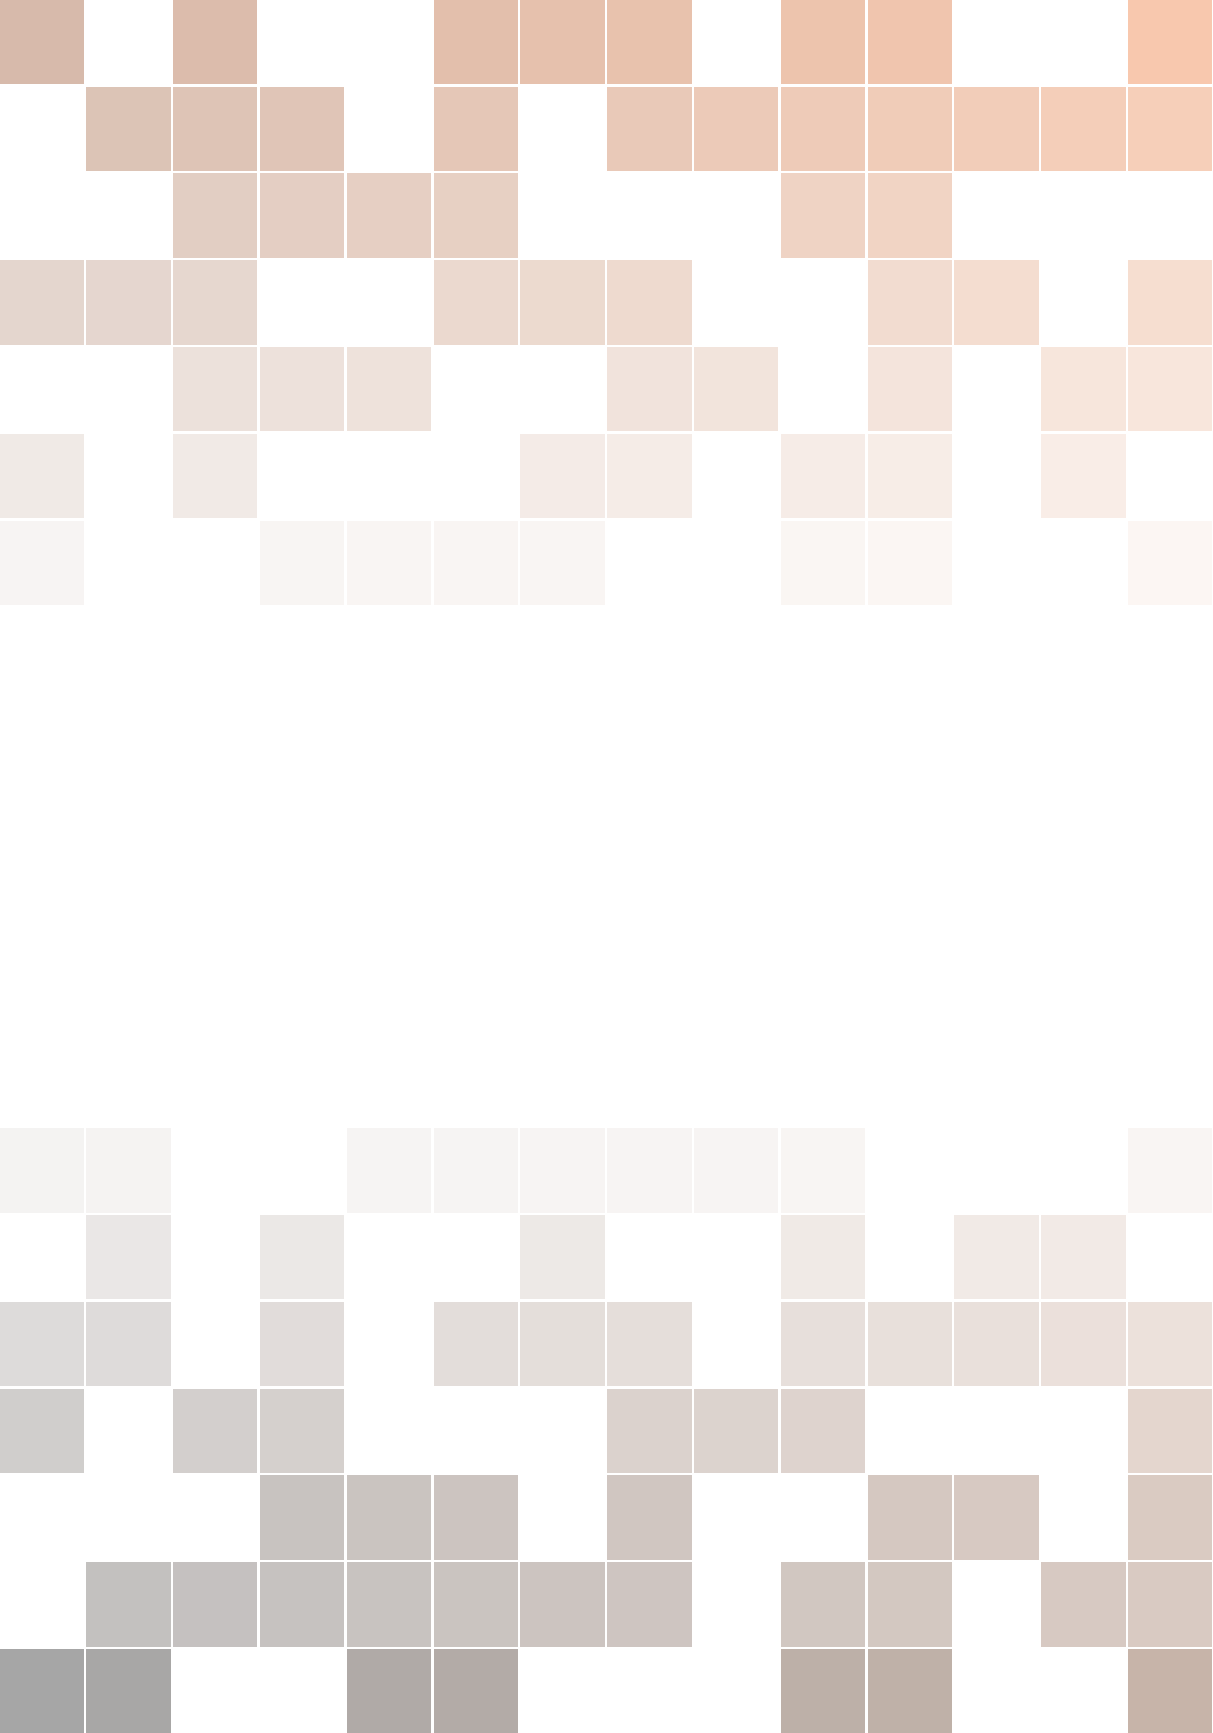
\includegraphics[width=\paperwidth]{images/background}}; % Background image
%\textsl{}
%      \draw[anchor=north] (midpoint) node [fill=ocre!30!white,fill opacity=0.6,text opacity=1,inner sep=1cm]{\Huge\centering\bfseries\sffamily\parbox[c][][t]{\paperwidth}{\centering Coding Interview Essentials\\[15pt] % Book title
%      {\Large - }\\[20pt] % Subtitle
%      {\huge Davide Spataro}}}; % Author name
%    \end{tikzpicture}};
%\end{tikzpicture}
%\vfill
%\endgroup


\includepdf[pages={2},fitpaper=true]{images/book_covers1.pdf}


	\usechapterimagefalse % If you don't want to include a chapter image, use this to toggle images off - it can be enabled later with \usechapterimagetrue

	%\chapterimage{images/header} % Table of contents heading image
	
	\pagestyle{empty} % No headers
	
	\tableofcontents % Print the table of contents itself
	
	\lstlistoflistings
	%\listoffigures
	%\listoftables

	%\cleardoublepage % Forces the first chapter to start on an odd page so it's on the right
	
	%pagestyle{fancy} % Print headers again

	%!TEX root = ../main.tex
%%%%%%%%%%%%%%%%%%%%%%%%%%%%%%%%%%
% Links:
%
% Difficulty: Companies: 
%%%%%%%%%%%%%%%%%%%%%%%%%%%%%%%%%%


%\begin{figure} \centering
%   \includegraphics[width=\textwidth]{sources/remove_duplicated_sorted_array_inplace/images/example1}
%   \caption[Sample short cpation]{Sample Caption}.
%   \label{fig:remove_duplicated_sorted_array_inplace:example1} \end{figure}

\chapter{Remove duplicates in sorted array}
\label{ch:remove_duplicated_sorted_array_inplace}
\section*{Introduction}
Sorting and duplicates are the bread and butter of coding interview questions.
There are countless
problems that ask you to perform some task, or calculate an answer, where you are given either some form of sorted
input or there are duplicates involved.

In the problem described in this chapter, we are going to investigate
how we can remove duplicates from an already sorted collection of elements. This problem is easily solvable when you can use linear space but doing it \textit{in-place} and by only using constant space is slightly more challenging.




\section{Problem statement}
\begin{exercise}
\label{example:remove_duplicated_sorted_array_inplace:exercice1}
Write a function that takes a sorted array $I$ as input and returns the number of unique elements $u$ in it. 
The function should also cause all the unique elements of $I$ to appear in the first $u$ positions.



	%example1
	\begin{example}
		\label{example:remove_duplicated_sorted_array_inplace:example1}
		\hfill \\
		Given $I=\{1,1,2,2,3,3,4,5,6,6,6,6,7\}$ the function returns $7$ and $I$ is rearranged such
		that itself first $7$ elements are $\{1,2,3,4,5,6,7\}$.				
	\end{example}

	%example2
	\begin{example}
		\label{example:remove_duplicated_sorted_array_inplace:example2}
		\hfill \\
		Given $I=\{1,2,3,4\}$ the function returns $4$ and $I$ is rearranged such that its first $4$
		elements are $\{1,2,3,4\}$.	
	\end{example}
\end{exercise}

\section{Clarification Questions}

\begin{QandA}
	\item \begin{questionitem} \begin{question} Is the input array guaranteed to contain integers?   \end{question} 	 
    \begin{answered}
		\textit{Yes you can assume $I$ is an array of integers, but only if you are free to produce a generic solution that works for any type.}
	\end{answered} \end{questionitem}	
\end{QandA}

\section{Discussion}
\label{remove_duplicated_sorted_array_inplace:sec:discussion}
This problem behavior is remarkably similar to the function \inline{std::unique} from the STL library: it does not really remove any element from the input collection, instead, it rearranges the elements to divide the initial collection. 
The official documentation for \inline{std::unique} says that:

\quoteblock{It eliminates all except the first element from every consecutive group of equivalent elements from a range and returns a past-the-end iterator for the new logical end of the range. Removing is done by shifting the elements in the range in such a way that elements to be erased are overwritten. The relative order of the elements that remain is preserved and the physical size of the container is unchanged. Iterators pointing to an element between the new logical end and the physical end of the range are still dereferenceable, but the elements themselves have unspecified values.}

As we can see, \inline{std::unique} does not really remove or erase any element from the input collection. 
What it does instead is rearrange the elements such that the initial collection is divided into
two parts:
\begin{enumerate}
	\item the first (from the left) containing only the unique elements;
	\item the second where the duplicate elements are moved to (possibly empty).
\end{enumerate}


This function is often used in real-life applications paired with \href{https://en.cppreference.com/w/cpp/container/vector/erase2}{\inline{std::erase}} to delete the second part of the newly
arranged collection when you actually want the duplicates removed.

Listing \ref{list:remove_duplicated_sorted_array_inplace_stl} shows how we can
solve this problem with a one-liner solution using \inline{std::unique} and \inline{std::distance} from the STL. 


\lstinputlisting[language=c++, caption={One-liner solution using \inline{std::unique}.},label=list:remove_duplicated_sorted_array_inplace_stl]{sources/remove_duplicated_sorted_array_inplace/remove_duplicated_sorted_array_inplace_solution3.cpp}

The code works by first invoking \inline{std::unique} and the entire array, which causes \inline{I} to be split into two parts as described above and returns an iterator to the the first element of the second part. 
\inline{std::distance} is then used to calculate the number of elements in the first part which is the final answer.

Being able to show you can use the standard library to solve a relatively complex problem is something any interviewer is going to appreciate, however, as important as making a good first impression is, this is unlikely to be enough to clear the interview round entirely. If you use this approach
during an actual interview, the interviewer is likely to ask you to implement \inline{std::unique} and \inline{std::distance} yourself.



\subsection{Linear space solution}

As mentioned in the introduction, it is quite easy to implement this problem when you can use
linear additional space. You can think of building a list $U$ of unique elements of $I$ by:

\begin{enumerate}
	\item insert the first element of $I$;
	\item insert at the back of $U$ every element of $I$ that is not equal to the last element of $U$.
\end{enumerate}



It is important to note that $U$ does not at any moment contain duplicates. Eventually, at the end of this process, $U$ contains an ordered list of all the unique elements in $I$. All we
have to do is copy $U$ into the first $|U|$ positions of $|I|$ and return $|U|$. The complexity
of this approach is linear in time and space, as in the worst-case scenario (when $I$ does not contain duplicates) we move the entire array $I$ into $U$, and then immediately copy $U$ back into $I$. An implementation of this approach is shown below in Listing
\ref{list:remove_duplicated_sorted_array_inplace_linearspace}.

\begin{figure} 
	\centering
   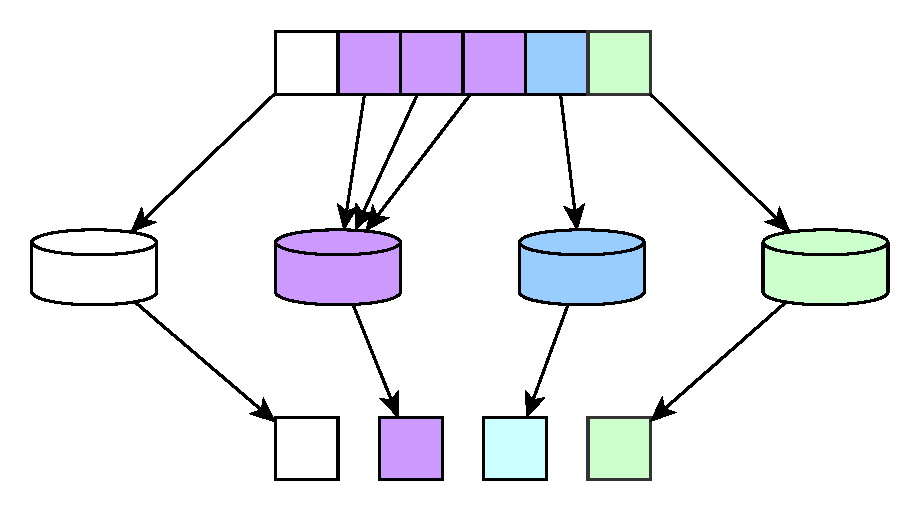
\includegraphics[width=\textwidth]{sources/remove_duplicated_sorted_array_inplace/images/intro}
   \caption[]{}
   \label{fig:remove_duplicated_sorted_array_inplace:example1} 
\end{figure}

\lstinputlisting[language=c++, caption={Linear time and space solution using \inline{std::std::unordered_set} to remember what elements have been already encountered.},label=list:remove_duplicated_sorted_array_inplace_linearspace]{sources/remove_duplicated_sorted_array_inplace/remove_duplicated_sorted_array_inplace_solution2.cpp}

\subsection{Constant Space}
\label{sec:remove_duplicated_sorted_array_inplace:constant_space}

Although we cannot do much better than spending linear time we can improve on the space used to the point where we only need a constant amount of it.
The key idea is that, because the array is sorted, equal elements will be next
to one another, therefore forming clusters of the same value. 
Eventually, $I$ has to be logically divided into
two subarrays where we only care about the content of the first part containing unique elements (no duplicates), as
there are no constraints on the content of the second part.

The algorithm proposed in this section uses a two pointer technique with which we
build the first half of $I$ one element at a time by looping through the
elements of $I$ and keeping track of two pointers:

\begin{itemize}
	\item $x$: a pointer to the last element of the first part of $I$;
	\item $y$: a pointer to the next element to be processed.
\end{itemize}

When the element pointed by $y$ is different from the element pointed by $x$, we know that we can add
$y$ to the first part of $I$. We can do that by copying $I_y$ into $I_{x+1}$ and incrementing both
$y$ and $x$ so that the next comparison would be among the last inserted element and a brand new unprocessed one.
If they are equal, however, the first part of $I$ is not going to grow and we can
safely ignore the element pointed by $y$ as we already have an instance of it (the value pointed by $X$) in the first half of $I$ already.

When all the elements of $I$ are processed ($y \geq |I|$) then the algorithm can be stopped. 
At this point
we know that $x$ is marking the end of the part of $I$ containing only unique elements. 
All we have to do is calculate and return its length. 

Listing \ref{list:remove_duplicated_sorted_array_inplace} shows an implementation of this idea.


\lstinputlisting[language=c++, caption={Linear time constant space solution.},label=list:remove_duplicated_sorted_array_inplace]{sources/remove_duplicated_sorted_array_inplace/remove_duplicated_sorted_array_inplace_solution1.cpp}

Note that with $x$ we have two important invariants:
\begin{enumerate}
	\item $x$ there are no duplicates among all the elements to the left of (including) $x$;
	\item $y$ is always larger than $x$.
\end{enumerate}

These invariants are true prior to entering the \inline{while} loop and they are true at the end of each and every iteration. It is also essential to note that the cells strictly between $x$ and $y$ can be overwritten as they must contain duplicates.

As already stated at the beginning of this section, the time complexity is linear but now, as opposed to the other solutions discussed so far, we use only constant space. 

Moreover, because we do not have to care about the state of the elements of $I$ after $x$,
we can use \href{https://en.cppreference.com/w/cpp/utility/move}{\inline{std::move}}\footnote{\inline{std::move} to indicate that an object t may be "moved from", i.e. allowing the efficient transfer of resources from t to another object without the need for an explicit copy.} to (potentially) avoid expensive copies.

Figure \ref{fig:remove_duplicated_sorted_array_inplace:example1_process} depicts the execution of this algorithm on the input of Example \ref{example:remove_duplicated_sorted_array_inplace:example1}, where the shaded part (the left side) of the array contains all the unique elements found so far (among all the elements to the left of $y$): $x$ is a pointer to the last element of this sequence and $y$ is a pointer to the element currently processed.


\begin{figure}
	\centering
	\vspace*{0.0in}
	\begin{subfigure}[t]{0.49\textwidth}
		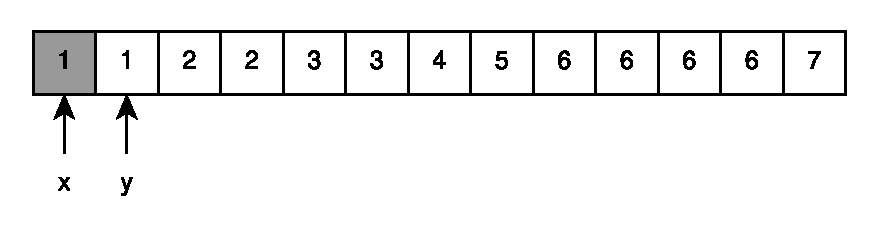
\includegraphics[width=1\linewidth]{sources/remove_duplicated_sorted_array_inplace/images/example1_1}
		\vspace*{-8mm}
		\caption{$I_x = I_y$. $y$ moved forward.}
		\label{fig:remove_duplicated_sorted_array_inplace:example1_1}
	 \end{subfigure}
	 \hfill
	 \begin{subfigure}[t]{0.49\textwidth}
		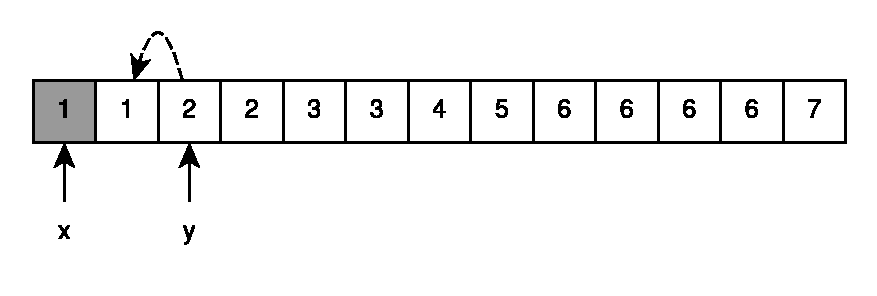
\includegraphics[width=1\linewidth]{sources/remove_duplicated_sorted_array_inplace/images/example1_2}
		\vspace*{-8mm}
		\caption{$1 = I_x \neq I_y = 2$. $I_y$ copied into $I_{x+1}$. $y$ and $x$ are moved forward.}
		\label{fig:remove_duplicated_sorted_array_inplace:example1_2}
	 \end{subfigure}
	 \hfill
	 \begin{subfigure}[t]{0.49\textwidth}
		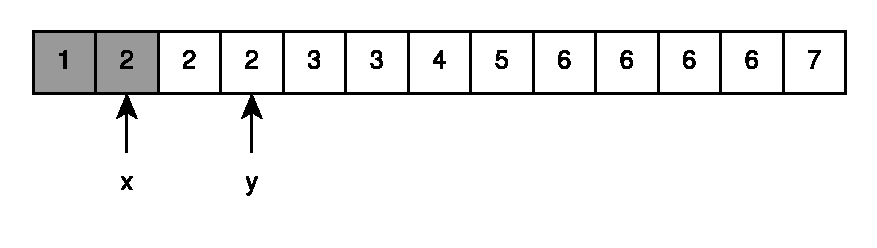
\includegraphics[width=1\linewidth]{sources/remove_duplicated_sorted_array_inplace/images/example1_3}
		\vspace*{-8mm}
		\caption{$I_x = I_y$. $y$ only moved forward.}
		\label{fig:remove_duplicated_sorted_array_inplace:example1_3}
	 \end{subfigure}
	 \hfill
	 \begin{subfigure}[t]{0.49\textwidth}
		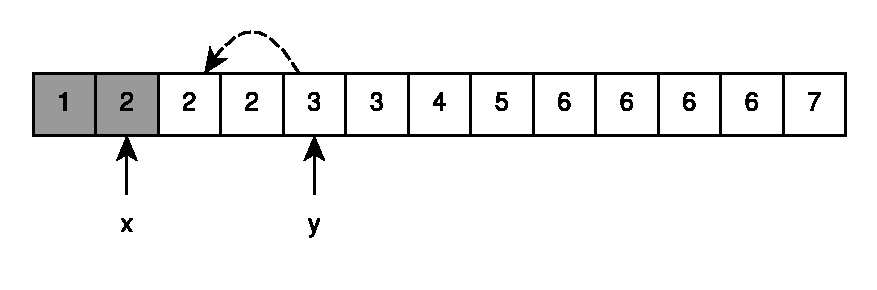
\includegraphics[width=1\linewidth]{sources/remove_duplicated_sorted_array_inplace/images/example1_4}
		\vspace*{-8mm}
		\caption{$2 = I_x \neq I_y = 3$. $I_y$ copied into $I_{x+1}$. $y$ and $x$ are moved forward.}
		\label{fig:remove_duplicated_sorted_array_inplace:example1_4}
	 \end{subfigure}
	 \hfill
	 \begin{subfigure}[t]{0.49\textwidth}
		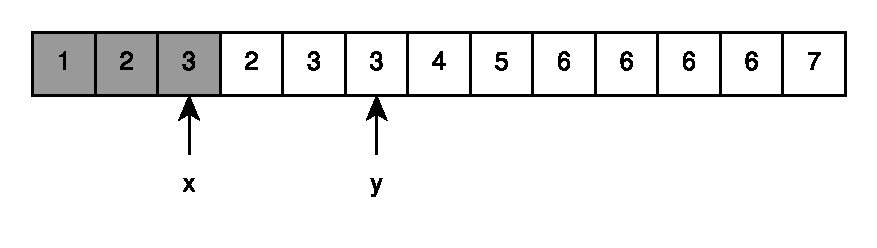
\includegraphics[width=1\linewidth]{sources/remove_duplicated_sorted_array_inplace/images/example1_5}
		\vspace*{-8mm}
		\caption{$I_x = I_y$. $y$ moved forward.}
		\label{fig:remove_duplicated_sorted_array_inplace:example1_5}
	 \end{subfigure}
	 \hfill
	 \begin{subfigure}[t]{0.49\textwidth}
		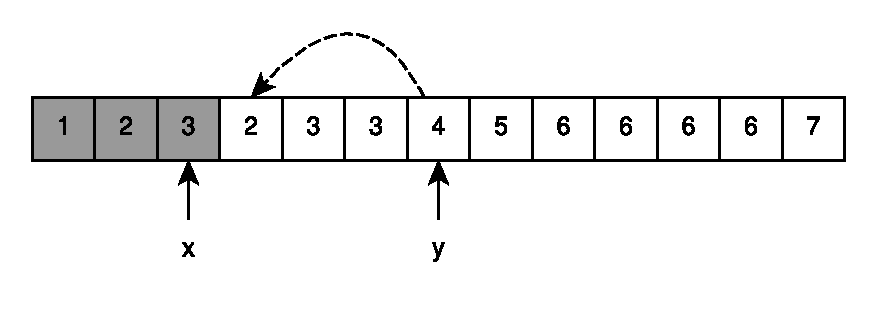
\includegraphics[width=1\linewidth]{sources/remove_duplicated_sorted_array_inplace/images/example1_7}
		\vspace*{-8mm}
		\caption{$3 = I_x \neq I_y = 4$. $I_y$ copied into $I_{x+1}$. $y$ and $x$ are moved forward.}
		\label{fig:remove_duplicated_sorted_array_inplace:example1_6}
	 \end{subfigure}
	 \hfill
	 \begin{subfigure}[t]{0.49\textwidth}
		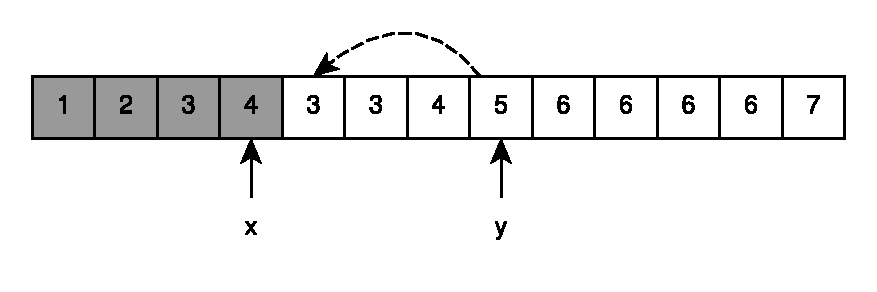
\includegraphics[width=1\linewidth]{sources/remove_duplicated_sorted_array_inplace/images/example1_8}
		\vspace*{-8mm}
		\caption{$4 = I_x \neq I_y = 5$. $I_y$ copied into $I_{x+1}$. $y$ and $x$ are moved forward.}
		\label{fig:remove_duplicated_sorted_array_inplace:example1_6}
	 \end{subfigure}
	 \hfill
	 \begin{subfigure}[t]{0.49\textwidth}
		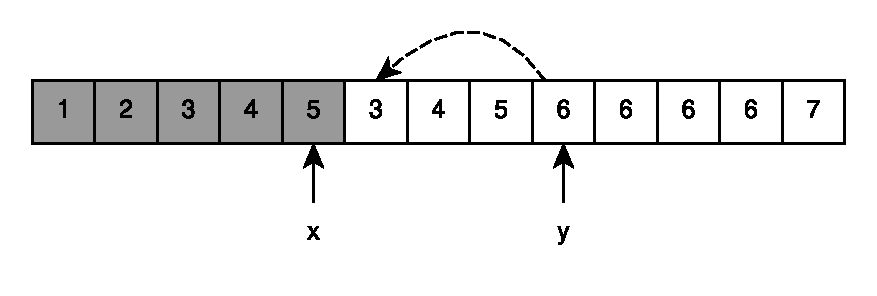
\includegraphics[width=1\linewidth]{sources/remove_duplicated_sorted_array_inplace/images/example1_10}
		\vspace*{-8mm}
		\caption{$5 = I_x \neq I_y = 6$. $I_y$ copied into $I_{x+1}$. $y$ and $x$ are moved forward.}
		\label{fig:remove_duplicated_sorted_array_inplace:example1_6}
	 \end{subfigure}
	 \hfill
	 \begin{subfigure}[t]{0.49\textwidth}
		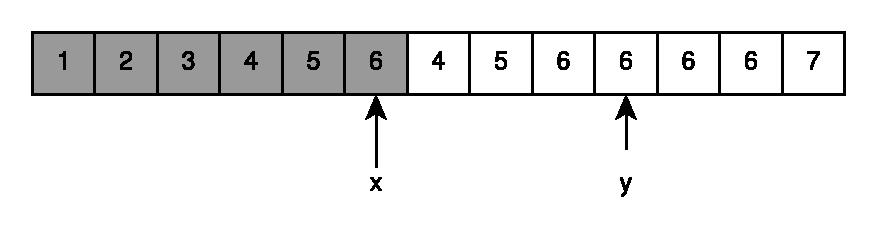
\includegraphics[width=1\linewidth]{sources/remove_duplicated_sorted_array_inplace/images/example1_11}
		\vspace*{-8mm}
		\caption{$I_x = I_y$. $y$ moved forward.}
		\label{fig:remove_duplicated_sorted_array_inplace:example1_6}
	 \end{subfigure}
	 \hfill
	 \begin{subfigure}[t]{0.49\textwidth}
		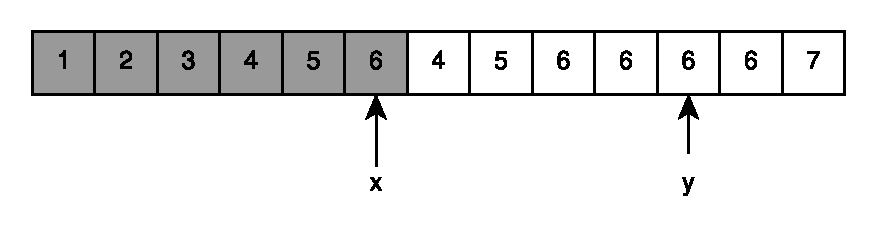
\includegraphics[width=1\linewidth]{sources/remove_duplicated_sorted_array_inplace/images/example1_12}
		\caption{$I_x = I_y$. $y$ moved forward.}
		\label{fig:remove_duplicated_sorted_array_inplace:example1_6}
	 \end{subfigure}
	 \hfill
	 \begin{subfigure}[t]{0.49\textwidth}
		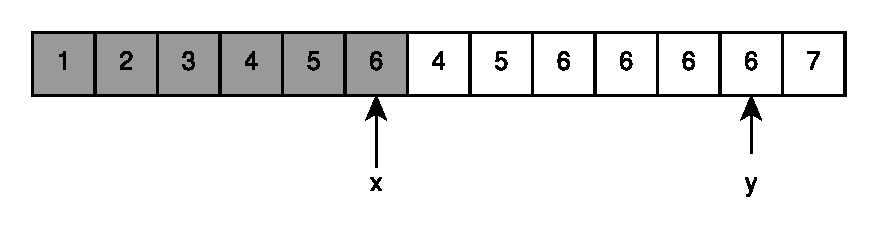
\includegraphics[width=1\linewidth]{sources/remove_duplicated_sorted_array_inplace/images/example1_13}
		\vspace*{-8mm}
		\caption{$I_x = I_y$. $y$ moved forward.}
		\label{fig:remove_duplicated_sorted_array_inplace:example1_6}
	 \end{subfigure}
	 \hfill
	 \begin{subfigure}[t]{0.49\textwidth}
		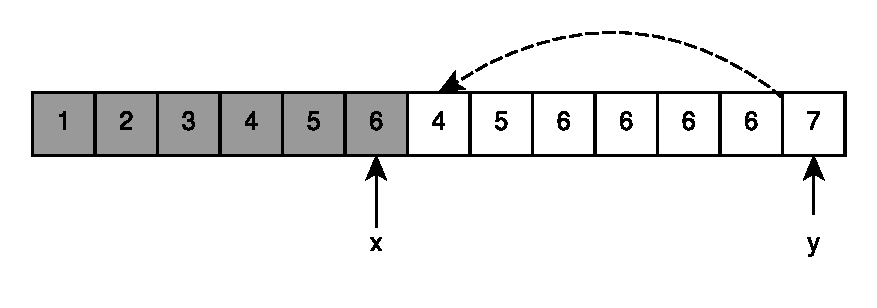
\includegraphics[width=1\linewidth]{sources/remove_duplicated_sorted_array_inplace/images/example1_14}
		\vspace*{-8mm}
		\caption{$6 = I_x \neq I_y = 7$. $I_y$ copied into $I_{x+1}$. $y$ and $x$ are moved forward.}
		\label{fig:remove_duplicated_sorted_array_inplace:example1_6}
	 \end{subfigure}
	 \hfill
	 \begin{subfigure}[t]{0.49\textwidth}
		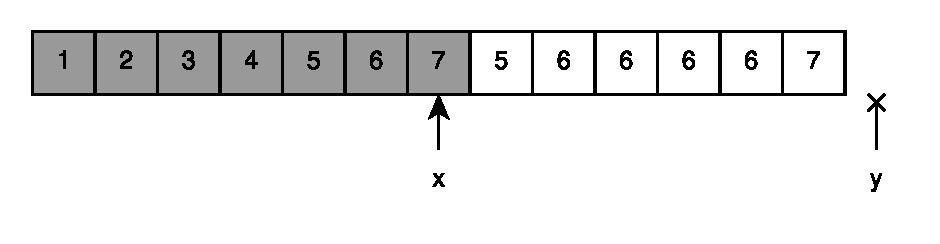
\includegraphics[width=1\linewidth]{sources/remove_duplicated_sorted_array_inplace/images/example1_15}
		\vspace*{-8mm}
		\caption{$y$ is outside the range of valid elements of $I$. The algorithm stops.}
		\label{fig:remove_duplicated_sorted_array_inplace:example1_6}
	 \end{subfigure}
\caption{Execution of the algorithm implemented in Listing
 \ref{list:remove_duplicated_sorted_array_inplace} on the input of the Example
 \ref{example:remove_duplicated_sorted_array_inplace:example1}. The shaded part of the array
 contains all the unique elements processed so far. $x$ is a pointer to the last element of this
 sequence. $y$ is a pointer to the element currently processed.}
\label{fig:remove_duplicated_sorted_array_inplace:example1_process}
\end{figure}

\section{Common Variations}
\subsection{Max $2$ duplicates allowed}
In this section, we will have a look at a common variation of the main problem of this lesson, which differs from it on the basis that each element can now appear at \textbf{most twice} in the final rearrangement of $I$.

\begin{exercise}
Write a function that  -  given a sorted array $I$  - removes all the 
duplicates in such a way that an element appears \textbf{at most twice} and with all the valid elements being located at the beginning of $I$ itself.
The function returns the number of valid elements in $I$.
	
	\label{example:remove_duplicated_sorted_array_inplace:exercice2}
	
		%example1
		\begin{example}
			\label{example:remove_duplicated_sorted_array_inplace_variation1:example1}
			\hfill \\
			Given $I=\{1,1,2,2,3,3,4,5,6,6,6,6,7\}$ the function returns $11$ and $I$ is rearranged such
			that itself first $11$ elements are $\{1,1,2,2,3,3,4,5,6,6,7\}$.				
		\end{example}
	
		%example2
		\begin{example}
			\label{example:remove_duplicated_sorted_array_inplace_variation1:example2}
			\hfill \\
			Given $I=\{1,2,3,4\}$ the function returns $4$ and $I$ is rearranged such that its first $4$
			elements are $\{1,2,3,4\}$.	
		\end{example}
\end{exercise}

\subsection{Discussion}

This variant can be solved with minimal changes to the solution presented for the main problem.
We can modify the code shown in the Section \ref{sec:remove_duplicated_sorted_array_inplace:constant_space} so that we keep track of the number of repetitions we have already inserted for a given element.
This can be implemented as shown in Listing \ref{list:remove_duplicated_sorted_array_inplace_max_two}.

\lstinputlisting[language=c++, caption={Linear time constant space solution to the variation where at most two duplicates are allowed.},label=list:remove_duplicated_sorted_array_inplace_max_two]{sources/remove_duplicated_sorted_array_inplace/remove_duplicated_sorted_array_inplace_solution4.cpp}


Note that the meaning of the variables $x$ and $y$ did not change, and that here we use the variable \inline{consecutive} to keep track of the number of times the element pointed by \inline{x} appears in the array \inline{A}. 
If the element pointed by \inline{y} is equal to the element pointed by \inline{x} (we have a duplicate), then we decide whether to insert it or not based on the value of the variable \inline{consecutive}:
\begin{itemize}
	\item If it appears already more than $1$ times we discard it;
	\item otherwise, we copy it to the cell at index $x+1$ and increment \inline{consecutive}.
\end{itemize}

The time and space complexity of this approach is $O(|I|)$ and $O(1)$, respectively.

\subsection{Max $k$ duplicates allowed}
This variation is also a quite common and is basically a generalization of the problems above where now each element can appear $k$ times.
Note that when $k= 1$ and $k=2$ this problem is equivalent to the Problems \ref{example:remove_duplicated_sorted_array_inplace:exercice1} and \ref{example:remove_duplicated_sorted_array_inplace:exercice2}.
The solution for this variation is not discussed here as it can be easily derived from the solution to the Problem \ref{example:remove_duplicated_sorted_array_inplace:exercice1}.

\begin{exercise}
Write a function that  - given a sorted array $I$  - removes all the 
duplicates in such a way an element appears at most twice and with all the valid elements being located at the beginning of the $I$ itself.
The function returns the number of valid elements in $I$.
	
	\label{example:remove_duplicated_sorted_array_inplace_variation:exercice3}
	
		%example1
		\begin{example}
			\label{example:remove_duplicated_sorted_array_inplace_variation2:example1}
			\hfill \\
			Given $I=\{1,1,2,2,3,3,4,5,6,6,6,6,7\}$ and $k=3$ the function returns $12$ and $I$ is rearranged such
			that itself first $1$ elements are $\{1,1,2,2,3,3,4,5,6,6,6,7\}$. Notice the extra $6$ w.r.t. the Example \ref{example:remove_duplicated_sorted_array_inplace_variation1:example1}.
		\end{example}
	
		%example2
		\begin{example}
			\label{example:remove_duplicated_sorted_array_inplace_variation2:example2}
			\hfill \\
			Given $I=\{1,1,1,1,1,1,1,2,2,3,3,3,4,4\}$ and $k=5$ the function returns $13$ and $I$ is rearranged such that its first $13$
			elements are $\{1,1,1,1,1,2,2,3,3,3,3,4,4\}$.	
		\end{example}
	\end{exercise}
	%!TEX root = ../main.tex
%%%%%%%%%%%%%%%%%%%%%%%%%%%%%%%%%%
% Links:
%
% Difficulty: Companies: 
%%%%%%%%%%%%%%%%%%%%%%%%%%%%%%%%%%


%\begin{figure} \centering
%   \includegraphics[width=\textwidth]{sources/remove_all_occurrences_unsorted_array_inplace/images/example1}
%   \caption[Sample short cpation]{Sample Caption}.
%   \label{fig:remove_all_occurrences_unsorted_array_inplace:example1} \end{figure}

\chapter{Remove all occurrences -  unsorted array}
\label{ch:remove_all_occurrences_unsorted_array_inplace}
\section*{Introduction}
The problem covered in this chapter asks us to implement a common operations: removeing all
elements satisfying specific criterium from a collection. This problem has many similarities to
the one discussed in Chapter \ref{ch:remove_duplicated_sorted_array_inplace} and as a consequence
they share the same general approach to their solution. 

There are many variations of this problem but the most common being  where the
collection is a simple array or a vector of integers and we are asked to remove all the elements
equal to a given integer. On this ocassion, however,  we will discuss a more generalized version where the 
collection is of a generic type \inline{T} and the criterium is given in the form of a unary
function returning a boolean\footnote{This type of function is commonly known as
\textit{predicates}.}. 

If you are asked to solve this particular problem version during an interview, you should be able to easily specialise what is discussed here in the moment.

\section{Problem statement}
\begin{exercise}
\label{example:remove_all_occurrences_unsorted_array_inplace:exercice1}
Write a function that -  given a collection $I$ of elements of type \inline{T}
 and a predicate function
 $p$ with signature \inline{bool(const T&)} -  rearranges $I$ in such a way that all the $0 \leq k
 \leq |I|$ elements satisfying $p$ in $I$ are moved to the front. The function should returns $k$.

 Moreover, the relative order of the elements  satisfying $p$ should be preserved. If both elements
 at indices $n$ and $m$ satisfy the predicate $p$  and $I_n$ comes before $I_m$ then when the
 function returns, their relative order is unchanged albeit they both might be moved to new
 locations.
 
	%example1
	\begin{example}
		\label{example:remove_all_occurrences_unsorted_array_inplace:example1}
		\hfill \\
		Given $I = \{{4, 1, 1, 2, 1, 3\}}$ and a function $p$ returning true if its input argument is an even number, false otherwise, the function returns $4$. The first $4$ elements of $I$ are $\{1,1,1,3\}$. 
		
	\end{example}

	\begin{example}
		\label{example:remove_all_occurrences_unsorted_array_inplace:example2}
		\hfill \\
		Given $I = \{4, 1, 1, 2, 1, 3\}$ and a function $p$ returning true if its input argument is odd, the function returns $2$. At this point, the first $2$ elements of $I$ are $\{4,2\}$. 
		
	\end{example}
\end{exercise}

\section{Clarification Questions}

\begin{QandA}
	\item \begin{questionitem} \begin{question} What should the content be of $I$ from index $k+1$ and after?  \end{question} 	 
    \begin{answered}
		\textit{There are no constraints on the content of those cells of $I$.}
	\end{answered} \end{questionitem}
	
\end{QandA}

\section{Discussion}
\label{remove_all_occurrences_unsorted_array_inplace:sec:discussion}
This problem could be restated as: \textit{Implement the
\inline{remove_if}\footnote{\url{https://en.cppreference.com/w/cpp/algorithm/remove}}} function from
the C++ STL. So it would not be surprising if, during an interview,  it could come-up as a
one-liner as  shown in Listing \ref{list:remove_all_occurrences_unsorted_array_inplace:STL}
\footnote{Notice the similarities with Listing \ref{list:remove_duplicated_sorted_array_inplace_stl} for the problem in Chapter \ref{ch:remove_duplicated_sorted_array_inplace}}.

\lstinputlisting[language=c++, caption={One-liner solution using the STL functions \inline{distance} and \inline{remove_if}},label=list:remove_all_occurrences_unsorted_array_inplace:STL]{sources/remove_all_occurrences_unsorted_array_inplace/remove_all_occurrences_unsorted_array_inplace_solution1.cpp}


This algorithm has a linear time and constant space complexity, which is pretty much as good as it gets considering you must at least read all the elements in the input array. 
It is worth mentioning, however, that  if you present this solution to an interviewer you can expect to be asked to implement the logic behind \inline{std::remove_if}
 itself as this is the core of the problem. 

\subsection{Linear time and linear space solution}
\label{remove_all_occurrences_unsorted_array_inplace:sec:bruteforce}
There is a straightforward way of solving this problem that has the added benefit of occupying
only a couple of lines and of being very clear and simple. The idea is that we can use an additional
linear amount of space to temporarily store the valid (dissatisfying the predicate \inline{p}
) elements, and in a subsequent
phase move them to the front of \inline{I}
. Listing \ref{list:remove_all_occurrences_unsorted_array_inplace:copy} shows a possible implementation of this idea.

\lstinputlisting[language=c++, caption={Linear space solution using the \inline{std::copy} family of functions from the STL.},label=list:remove_all_occurrences_unsorted_array_inplace:copy]{sources/remove_all_occurrences_unsorted_array_inplace/remove_all_occurrences_unsorted_array_inplace_solution2.cpp}


This solution only works correctly for types that can be copied. As such, the interviewer could
 ask you to fix this; in which case you can loop over \inline{I}
 and \inline{temp}
 and
\href{https://en.cppreference.com/w/cpp/utility/move}{\inline{move}
}\footnote{\inline{std::move}
 is used to indicate that an object t may be "moved from", i.e. allowing the efficient transfer of resources from t to another object without the need for an explicit copy.}
 the elements around instead.



\subsection{Linear time and constant space solution}
\label{remove_all_occurrences_unsorted_array_inplace:sec:constant_space}

The idea discussed in Section \ref{remove_all_occurrences_unsorted_array_inplace:sec:bruteforce} can quite easily be modified so that we avoid using additional linear
space. We could use \inline{std::move} the elements of $I$ into $I$ itself in the same way as we did for the problem covered in Chapter \ref{ch:remove_duplicated_sorted_array_inplace}
while discussing the solution \ref{list:remove_duplicated_sorted_array_inplace}. 

Here we use exactly the same approach of two pointers $x$ and $y$:
\begin{enumerate}
	\item  $x$ keeps track of the new front to $I$. It points to the end of the portion of $I$ (starting at index $0$ and ending at $x-1$) containing all the valid elements found so far;
	\item $y$ is a pointer to the next element not yet processed in $I$.
\end{enumerate}

Listing \ref{list:remove_all_occurrences_unsorted_array_inplace:constant_space} implements this idea.

\lstinputlisting[language=c++, caption={Constant space solution using a two pointer approach.},label=list:remove_all_occurrences_unsorted_array_inplace:constant_space]{sources/remove_all_occurrences_unsorted_array_inplace/remove_all_occurrences_unsorted_array_inplace_solution3.cpp}



At the beginning of the execution the algorithm moves $x$ forward. All the valid elements that are already
at the front of $I$ stay untouched as they are already in the right locations.
At this point, $x$ points either to the first invalid element in $I$ or to one element past $I$.
In the second scenario, there is no more work to do. All the elements are valid to begin with, and the second \inline{while}

will not even start. $I$ is left unchanged.
In the first scenario, we will use $y$ to scan the remaining elements of $I$ past $x$, and we move each valid element we encounter 
into the location pointed by $x$. When this happens $x$ is moved forward as the portion of valid elements grew by one element. 

Notice that the invariant $x \leq y$ is always respected as:
\begin{itemize}
	\item it holds before the beginning of the loop;
	\item $x$ is incremented at the same rate or less compared to $y$.
\end{itemize}

At the end of this process, we are left with $y$ pointing to the one element past $I$ and $x$ pointing to one cell after the last valid element of the newly rearranged $I$.
	
	%%%%%%%%%%%%%%%%%%%%%%%%%%%%%%%%%%%%%%%%%%%%
	%               Appendices
	%%%%%%%%%%%%%%%%%%%%%%%%%%%%%%%%%%%%%%%%%%%%
	
	\chapter{Appendices}
	% @Author: Davide Spataro
% @Date:   2020-10-25 
% @Last Modified by:   Davide Spataro
% https://www.topcoder.com/community/competitive-programming/tutorials/dynamic-programming-from-novice-to-advanced/
% file:///home/knotman/Downloads/DYNAMIC_PROGRAMMING_-_ITS_PRINCIPLES_APPLICATIONS_.pdf
% http://smo.sogang.ac.kr/doc/bellman.pdf 
\section*{Dynamic Programming}
\label{sect:appendix:DP}

Dynamic programming (DP) is a popular technique for solving a certain class of
optimization problems efficiently and is accredited to the American Scientist
Richard Bellman\cite{bellman1954}. He conied the term DP in the context of
solving problems involving a serie of best decision one after the other. 
The word \textit{programming} can be a bit deceiving for
computer scientist of programmers in general but it has really little to do with
computer programming and it is infact intended as a set of rules to 
follow to solve a certain problem and it is refeered specifically to the
solution to find an optimal military schedule for logistics (and has more or
less the same meaning as linear programming or linear optimization).  These rules can of course be coded and
executed by a computer but can be easily followed on paper for instance. 
Dynamic programming is better thought as an optimization approach rather than an
method or framework where a complex optimization problem is transformed into a sequence of
smaller (and simpler) problems. The very essence of DP is its multi-stage
optimization procedure. DP does not provide directly with the
instruction on how to solve a particular problem, but instead provides a general
framework that requires creativity and non trivial effort/insights so that a
problem formulation can be adapted and casted within the DP framework bounds.
This is possibly the reason why DP is considered a rather hard topic and it is
particularly feared during interviews. 

This chapter is not intended to be a full treatement of DP, and we will
introduce and describe it to the level that is necessary to understand and
better tackle DP interview problems. For a more comprenshive material on DP
please refer to \cite{bellman1954, cormen2009}.

The gist of the DP approach is that we aim at breaking down a problem into
simpler sub-problems recursively. If it is possible to do so, then the problem
at hand is said to have the \textbf{optimal substructure} property i.e. it can
be solved by using optimal solution to subproblems. But having the optimal
substructure property alone is not enough to prefer a DP approach to another
when trying to solve the same problem. This is because DP really shines when a
problem also exposes the \textbf{overlapping subproblems} property i.e. when the
subproblems are reused several times. A classic example if the
Fibonacci Sequence. In order to calculate $F(n)$ we need to solve two subproblems:
$F(n-1)$ and $F(n-2)$ and adding them up. But for solving $F(n-1)$ we need to
solve $F(n-2)$ \textbf{again}. The value for the subproblem $F(n-2)$ is thus
reused and this makes the Fibonacci problem exposed the optimal substructure
property. 
Dynamic programming takes care of this fact by making sure of solving each
subproblem only once. Usually this can be achieved into two ways:
\begin{description}
    \item [Top-down] This is usually the easiest of the two, by being a direct
    derivation from the recursive formulation of the problem. If the problem can
    be formulated recursively in terms of solution then solution to subproblems
    can be \textit{memoized}\footnote{From the latin word \textit{memorandum}
    which means to be remembered. It is basically a way of remembering the
    result of a function for a certain set of inputs call by storing it in a
    cache.} in a cache. 
    When a subproblem is reused then the
    (potentially expensive) recursive call is avoided and the cached result is
    returned instead. 
    \item [Bottom-up] We can try to reformulate the problem by twisting and
    massaging  the  recursive formulation so that the subproblems are solved
    first (thus effectively removing the recursion) and build the solution to
    the bigger problem from the bottom. This is usually done by working in a
    sort of tabular form where entries of the table for larger problems are
    filled by using  entries for solution to smaller problems that we have
    already solved. For instance, when solving the problem of finding the
    $10^{th}$ Fibonacci number $F(10)$, we can start from the known values for
    $F(0)$ and $F(1)$ and working our way up to $F(2)$  by using $F(1)$ and
    $F(2)$. Once F(2) is ready we can move up to F(3), and so on when we have
    the values for $F(8)$ and $F(9)$ we proceed with calculating $F(10)$.
\end{description}

DP has found application in many field of science such as Control theory,
Bioinformatics AI and operations research. There are a number of problems in
computer science that can be solved by using DP such as the 
\begin{itemize}
    \item Longest Common (or increasing) Subsequence
    \item Weighted Interval Scheduling
    \item Chain Matrix Multiplication
    \item Subset sub
    \item String edit distance
    \item Coin change
    \item 0/1 knapsack problem
    \item Graph shortest path
\end{itemize}

In the next section we will shortly review a number of DP problem focusing on
the key ideas that allow a problem to be approached and solved  using DP.

\subsection*{Fibonacci Sequence}
Computing the $n^{th}$ number of the Fibonacci sequence is probably one of the
most common introductionary example of DP. The Fibonacci sequence recursive
formulation is ready to be solved using a top-down DP approach. Listing
\ref{list:app:dp:canonical} shows a C++ function that calculated the $n^{th}$ Fibonacci
number.
\lstinputlisting[language=c++, caption={Canonical recursive C++ implementation of a function returning the $n^{th}$ Fibonacci number.},label=list:app:dp:canonical]{/home/dspataro/git/algorithm_articles/sources/appendices/fibonacci_canonical.cpp}
Notice that for instance when $F(6)$ a call tree is produced where the same call
is repeated more than once as shown in the list below. $F(2)$ has been
calculated $5$ times!
\begin{itemize}
    \item $F(6) = F(5)+F(4)$
    \item $F(6) = (F(4)+F(3)) + (F(3)+F(2))$
    \item $F(6) = ((F(3)+F(2))+(F(2)+F(1))) + ((F(2)+F(1))+(F(1)+F(0)))$
    \item $F(6) = (((F(2)+F(1))+(F(1)+F(0)))+((F(1)+F(0))+F(1))) + (((F(1)+F(0))+F(1))+(F(1)+F(0)))$
    \item $F(6) = ((((F(1)+F(0))+F(1))+(F(1)+F(0)))+((F(1)+F(0))+F(1))) + (((F(1)+F(0))+F(1))+(F(1)+F(0)))$
\end{itemize}

Listing \ref{list:app:dp:fib} can be improved dramatically if we memoize the function calls
that have been already calculated. This way no duplicate work is done. W.r.t the
previous example, from the second time the value of $F(2)$ is needed, no
additional work is done, as the value in the cache is returned.
\lstinputlisting[language=c++, caption={Canonical recursive top-down Dynamic Programming C++ implementation of a function returning the $n^{th}$ Fibonacci number.},label=list:app:dp:fib]{/home/dspataro/git/algorithm_articles/sources/appendices/fibonacci_dp_top_down.cpp}

	%\section{Prefix sum}
\label{sect:appendix:prefix_sum}
In computer science, the prefix sum, cumulative sum, inclusive scan, or simply scan of a sequence of numbers x0, x1, x2, ... is a second sequence of numbers y0, y1, y2, ..., the sums of prefixes (running totals) of the input sequence:
	%% @Author: Davide Spataro
% @Date:   2020-03-30 17:18:14
% @Last Modified by:   Davide Spataro
% @Last Modified time: 2020-03-30 17:28:08
\section{Binary Search}
\label{sect:appendix:binary_search}
\lipsum{1}
    %%%%%%%%%%%%%%%%%%%%%%%%%%%%%%%%%%%%%%%%%%%%
	%               BIBLIOGRAPHY
	%%%%%%%%%%%%%%%%%%%%%%%%%%%%%%%%%%%%%%%%%%%%
	
	%\chapter*{Bibliography}
	\addcontentsline{toc}{chapter}{\textcolor{ocre}{Bibliography}}
	\printbibliography	
	
%%%%%%%%%%%%%%%%%%%%%%%%%%%%%%%%%%%%%%%%%%%%
%               INDEX
%%%%%%%%%%%%%%%%%%%%%%%%%%%%%%%%%%%%%%%%%%%%	
	\cleardoublepage
	\phantomsection
	\setlength{\columnsep}{0.75cm}
	\addcontentsline{toc}{chapter}{\textcolor{ocre}{Index}}
	\printindex


	%\backmatter

\end{document}
